%!TEX root = ../master.tex
\chapter{Background Research}\label{ch:bgres}

The background research in this chapter is based on acquiring answers to the initial problem statement and the two research questions. The research includes studies of state of the art artefacts, previous work and which methods they used. 


\section{Target Group Explained}\label{sec:TargetGroup}
The project's target group are people who are experienced with board games, maybe even Terra Mystica, and are 14 years old or above since this is the game's recommended age group. This is because Terra Mystica itself caters to people who have a certain amount of experience with board games or people who like to play complex games, as the game has a lot of rules to keep track of. The project does not aim to simplify the game's core, but rather streamline the game mechanics, and therefore players who are inexperienced with complex board games will not benefit, since Terra Mystica is not a simple game to play.

\section{Previous scientific work}
In this section, other attempts to digitally augment board games will be discussed.

Andersen et al. \citep{andersen_designing_2004} created "BattleBoard3D", a board game utilising physical and digital components. For their physical components they used flat squares with patterns that through Augmented Reality (AR) technologies will be recognised through a camera and/or Virtual Reality goggles. Their research was made to illustrate "design issues for AR board games".

Peitz et al. \citep{peitzWizards2006} created "Wizard's Apprentice", a computer-augmented board game. The game includes two roles: wizard and apprentice. All players but one play as apprentices guided by the wizard who acts as a negotiator and motivator. The software is written in Java and has several play modes. The game uses Radio-Frequency Identification (RFID) hardware to detect at which physical point the players are in the game. It sends this information through antennas to a laptop close by. The laptop projects this information to a screen that displays relevant information on each player's turn. The game board can be seen in Figure \ref{fig:peitz}.

Magerkurth et al. \citep{magStars} created "STARS", a ubiquitous computing platform for computer augmented tabletop games. This platform includes devices such as a game table, a wall display, PDAs, and audio devices. The purpose of this platform was to provide features that went beyond what normal board games are capable of, while still maintaining the experience of the players interacting as they would with a normal board game. The platform was also able to save game states with ID tags, remember complex rules so they would not slow down the pacing of a game, and make the game board react dynamically to interactions with the game and its pieces. Its software is developer-friendly so that creating rules and content could be prioritised over device integration and game board management. 

\begin{figure}[!h]
\centering	
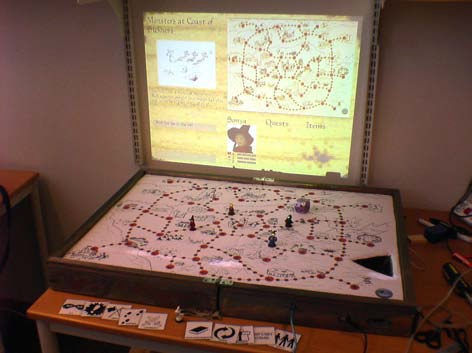
\includegraphics[width=0.5\textwidth]{peitz}
\caption{The Wizard's apprentice game board setup from \citep{peitzWizards2006}}
\label{fig:peitz}
\end{figure}

\section{Commercial competition}
Apart from previous scientific work, commercial board games have been released, existing on a spectrum ranging from completely digital to completely analogue. As our product will exist somewhere on this spectrum, these commercial solutions described below can be considered state of the art for this project.

On the digital end, the online collectible card game Hearthstone \citep{Hearthstone} (for Windows, OS X, Android and iOS), though completely virtual, has an interface which resembles a physical game board with cards and information on it. The user plays the game by dragging the cards onto the board from their 'hand' by way of using the cursor (when playing on a desktop computer), or by swiping with a finger (when playing on a smartphone or a tablet). The cards placed on the board can then be dragged to the cards they need to attack, etc. This swiping mechanism gives the game a tangible sense, making it resemble an analogue card game, even though no physical cards are involved.

There are also board games which integrate phone or tablet applications into the gameplay. One such game is XCOM: The Board Game \citep{XCOM}, which simulates an alien attack the players then have to repel. The game has a physical game board, cards and pieces, but also a companion app, which can be downloaded to a desktop computer or mobile device. The app is required in order to play the game. It tracks the time each player has to do certain tasks, as well as what actions the aliens will take. The game therefore still looks like a normal board game, but it has a built-in augmentation in the form of the app, which changes the way turn/task orders and time constraints are done in a board game.

Another example of a board game which incorporates digital media is the card game, Munchkin \citep{Munchkin}. The game itself is a card game that can be played without augmentation. However, an app has been released which assists a player in keeping track of their current level and their combat strength compared to the monster they're fighting. Apart from that, the app provides the player using it with a bonus in the game\citep{Munchkin}. This is an example of a board game which has an optional digital augmentation, but it is not necessary to play the game.

\section{Methods for evaluating and measuring key success criteria}
Andersen et al. \citep{andersen_designing_2004} evaluated their product on a group of 13 year old children. The goals were to "reveal issues concerning the game design in general, design of the physical pieces, the use of goggles versus screen display, and future evolvement." The children found the 3D projection of the characters through the goggles fascinating, although some fumbling with the game pieces occurred due to the nature of the goggles and placement of the webcam. This occurred less when they looked at the 3D figures on the screen, but this brought along the problem of shifting focus away from the board game.
Finally, the children found the small set of animations uninteresting after a while and suggested a higher number of animations were needed to keep interest.

Peitz et al. \citep{peitzWizards2006} performed an initial evaluation on 3 children aged 8-9 and a male adult player (37). The evaluation was based upon a template that evaluates the social adaptability of game divided into: "(...)spatial, temporal, social, and playability." The participants were observed for two hours and were thematically interviewed afterwards. The participants reported overall enjoyment and increased togetherness in the game, but the pacing of the game felt unfamiliar. The participants seemed to particularly react positively to the sound design. 

\section{Competitive analysis}
As shown by Andersen et al. \citep{andersen_designing_2004}, a solution to enhance a board game can be done through AR aided by either a screen or Virtual Reality (VR) goggles. Andersen et al. mention some drawbacks to both of their technologies. In the case of AR with a screen they note that while the screen gives the participants the ability to look their opponent in the eye, they are distracted by having to look away from the board game space, to look at the screen displaying the figures. Regarding the VR, they note that participants liked the ability to pick up a game piece and explore all sides of the 3D model through the goggles. The problem, as can be seen in Figure \ref{fig:andersen}, could be that the goggles take away from the non-verbal communication that board games tend to foster.

In \citep{peitzWizards2006}, Peitz et al. built a board together with RFID antennas and other hardware to detect certain points of the the players' progression. They note some positive things, as aforementioned, namely the increased feeling of togetherness and overall enjoyment. They follow a recipe many traditional board games follow: a tile progression. They simulate this with the dots throughout the map, which the "tokens" press down on and activate. They also note the relationship between wizard and apprentices works well, but note an interesting development in the dynamics when one of the children effectively demotes the adult, who has the role as wizard, and temporarily acts as a new wizard. They did not account for this, but mention it is within their design goals.

As for the commercial competition, the solutions utilise digital media to varying degrees, in some cases combining these elements with traditional board game elements such as a board or cards, bringing in the aforementioned feeling of togetherness identified by Peitz et al \citep{peitzWizards2006}. However, in these multi-media solutions, the digital aspects are not integrated physically into the game, but rather exist as an additional, separate 'piece' of the game in the form of a phone, tablet or a personal computer. There is an unutilised potential in combining digital and physical elements in such a way that the players can feel the unity board games provide without the barrier of a screen between them, but at the same time have a program handle some of the management of parts, reducing the amount of time players have to spend on that.

\begin{figure}[!h]
\centering	
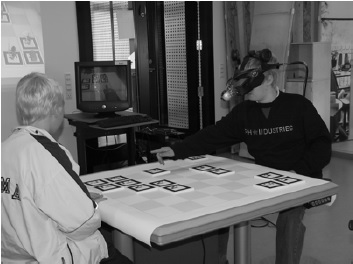
\includegraphics[width=0.5\textwidth]{andersen}
\caption{BattleBoard3D setup from Andersen et al.  \citep{andersen_designing_2004}}
\label{fig:andersen}
\end{figure}


\section{Terra Mystica}
\begin{figure}[h!]
\centering 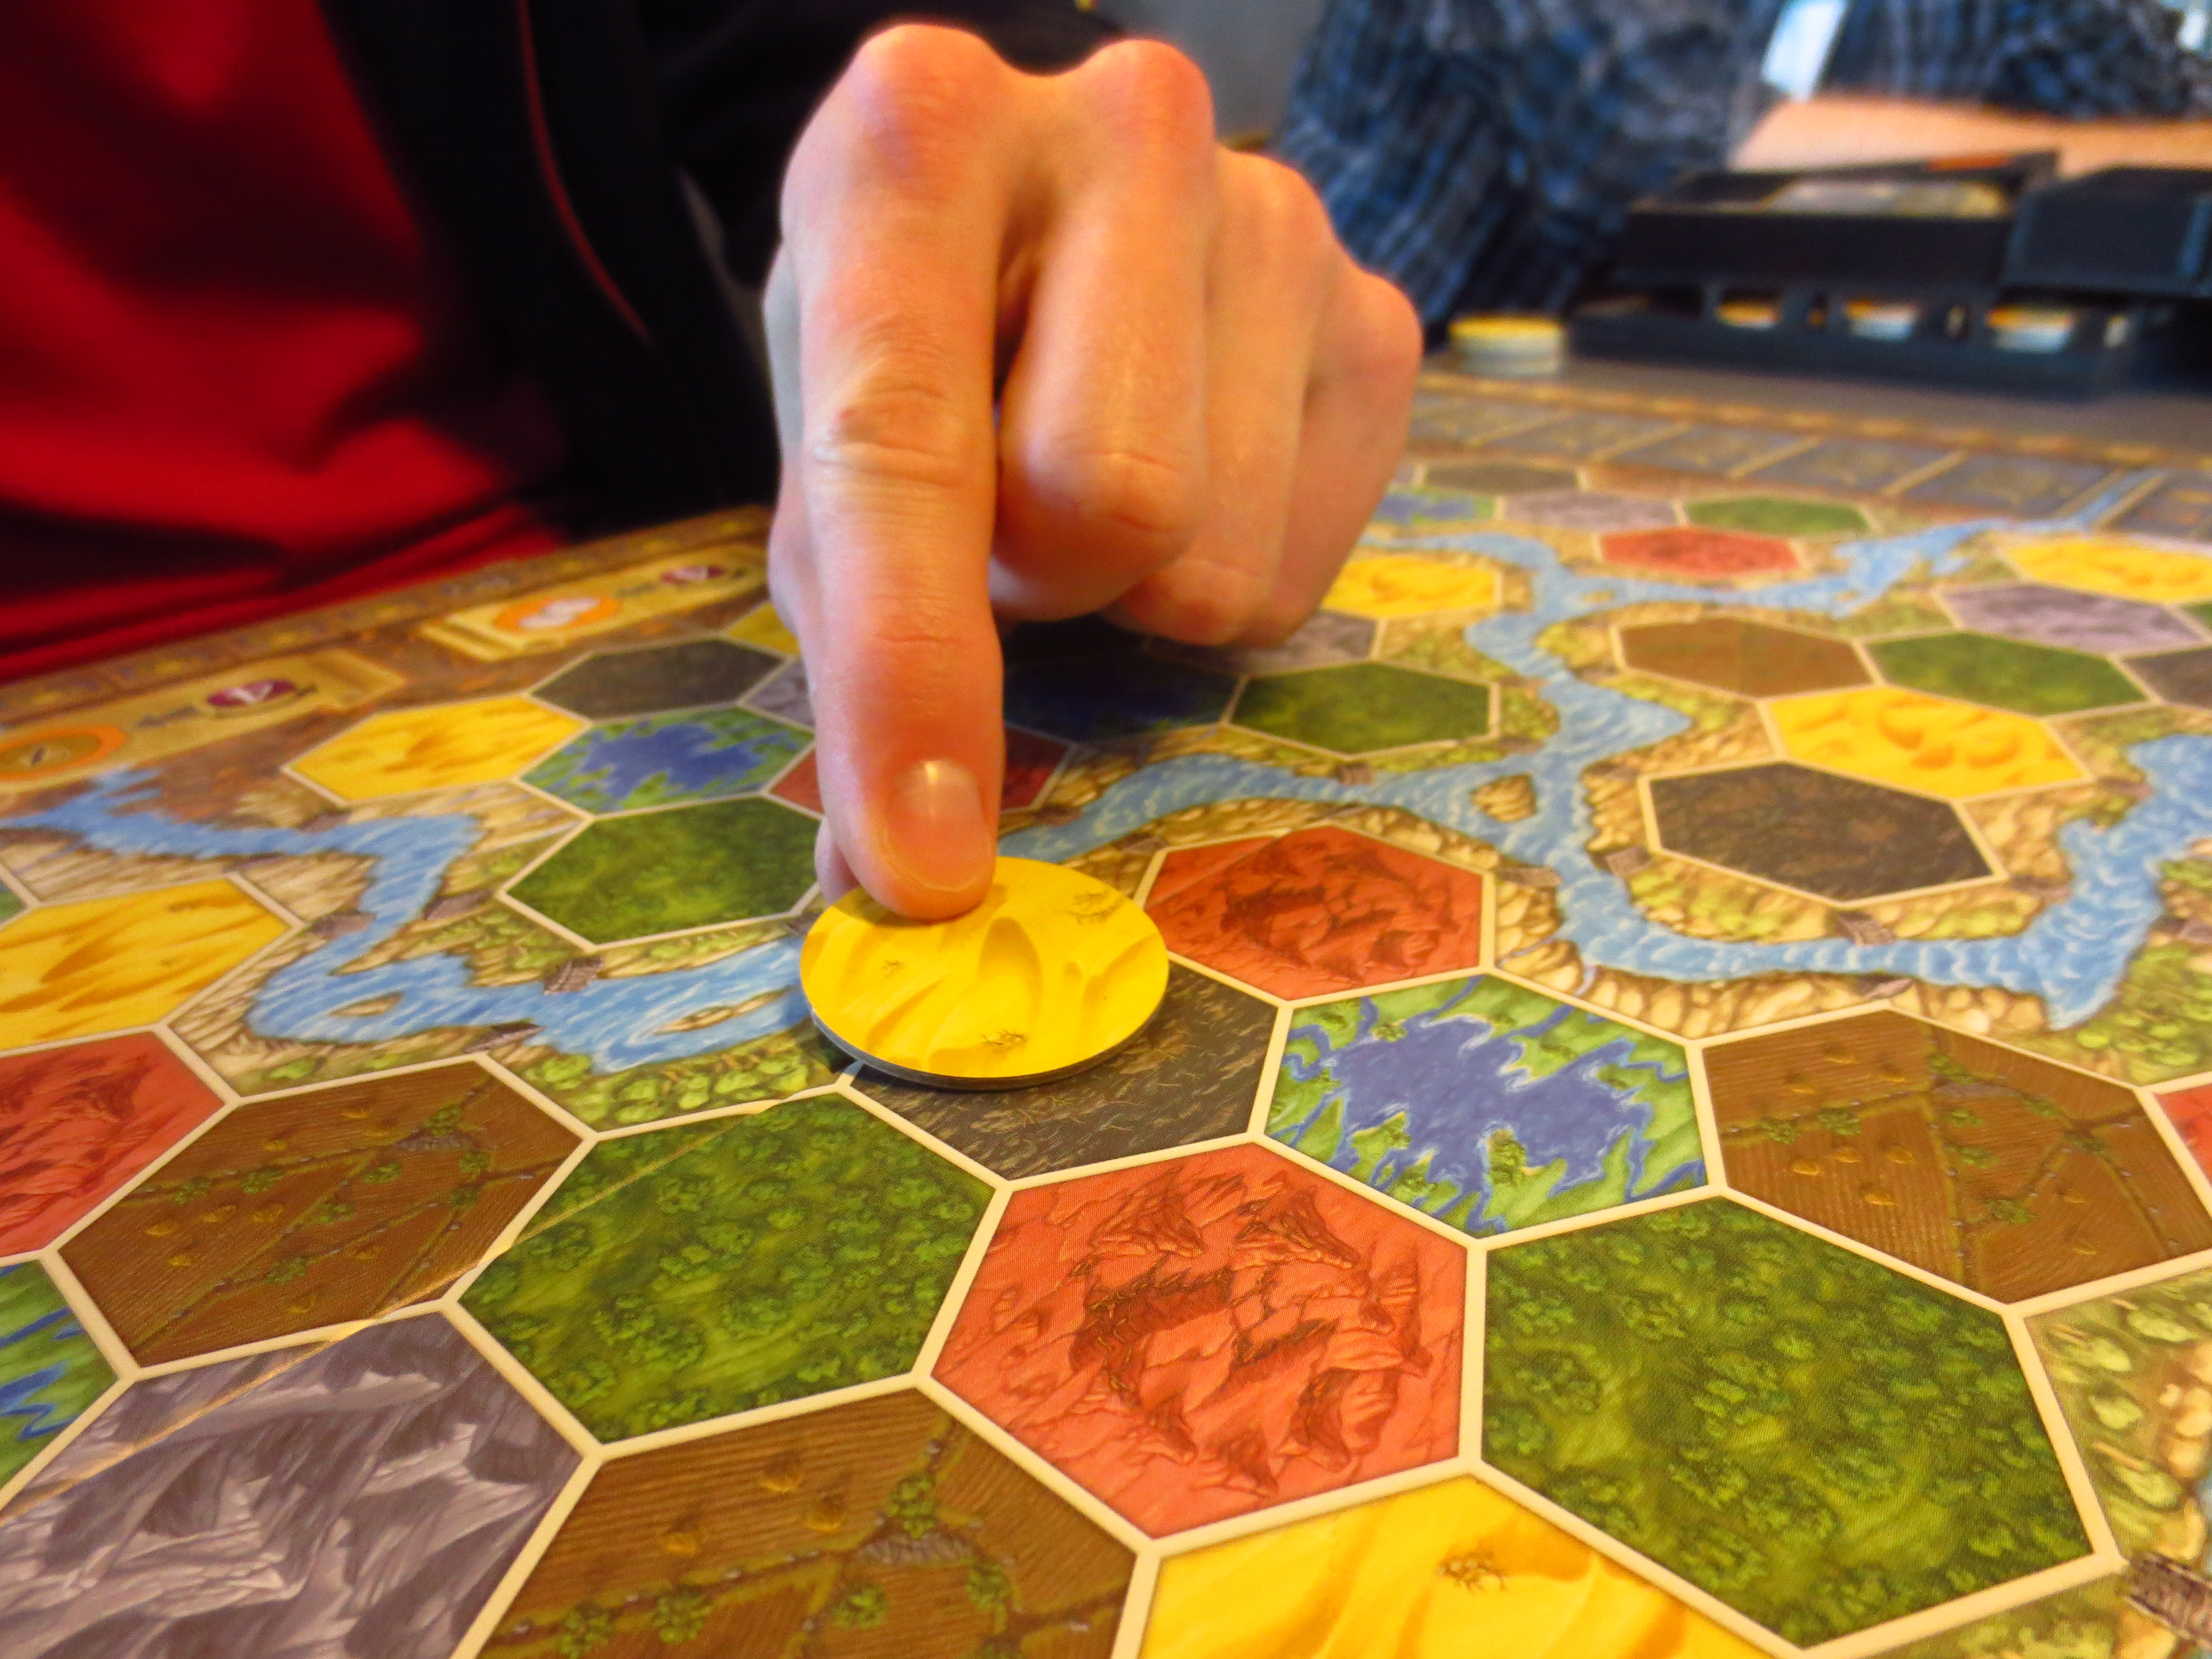
\includegraphics[width=0.5\textwidth]{TerraformingAction}
\caption{How to terraform in the board game \label{Fig:TerraformingAction}}
\end{figure}
Terra Mystica is a game that utilises a lot of different game pieces for different tasks. One of the tasks that use a lot of pieces is the task of terraforming a terrain into the faction's home terrain. Those terrain pieces are usually gathered in a big pile, where all pieces have a different type of terrain on each side. Alternatively, the players can gather a pile each with their own terrain on them, eliminating the need to search for a new piece every time you terraform. However, in some games, a player can terraform so much that they run out of pieces with which to terraform. This problem could be solved though an interactive board which removes the terrain pieces, and instead just changes the board itself. This way, there is no way to run out of terraforming pieces.
\begin{figure}[h!]
\centering 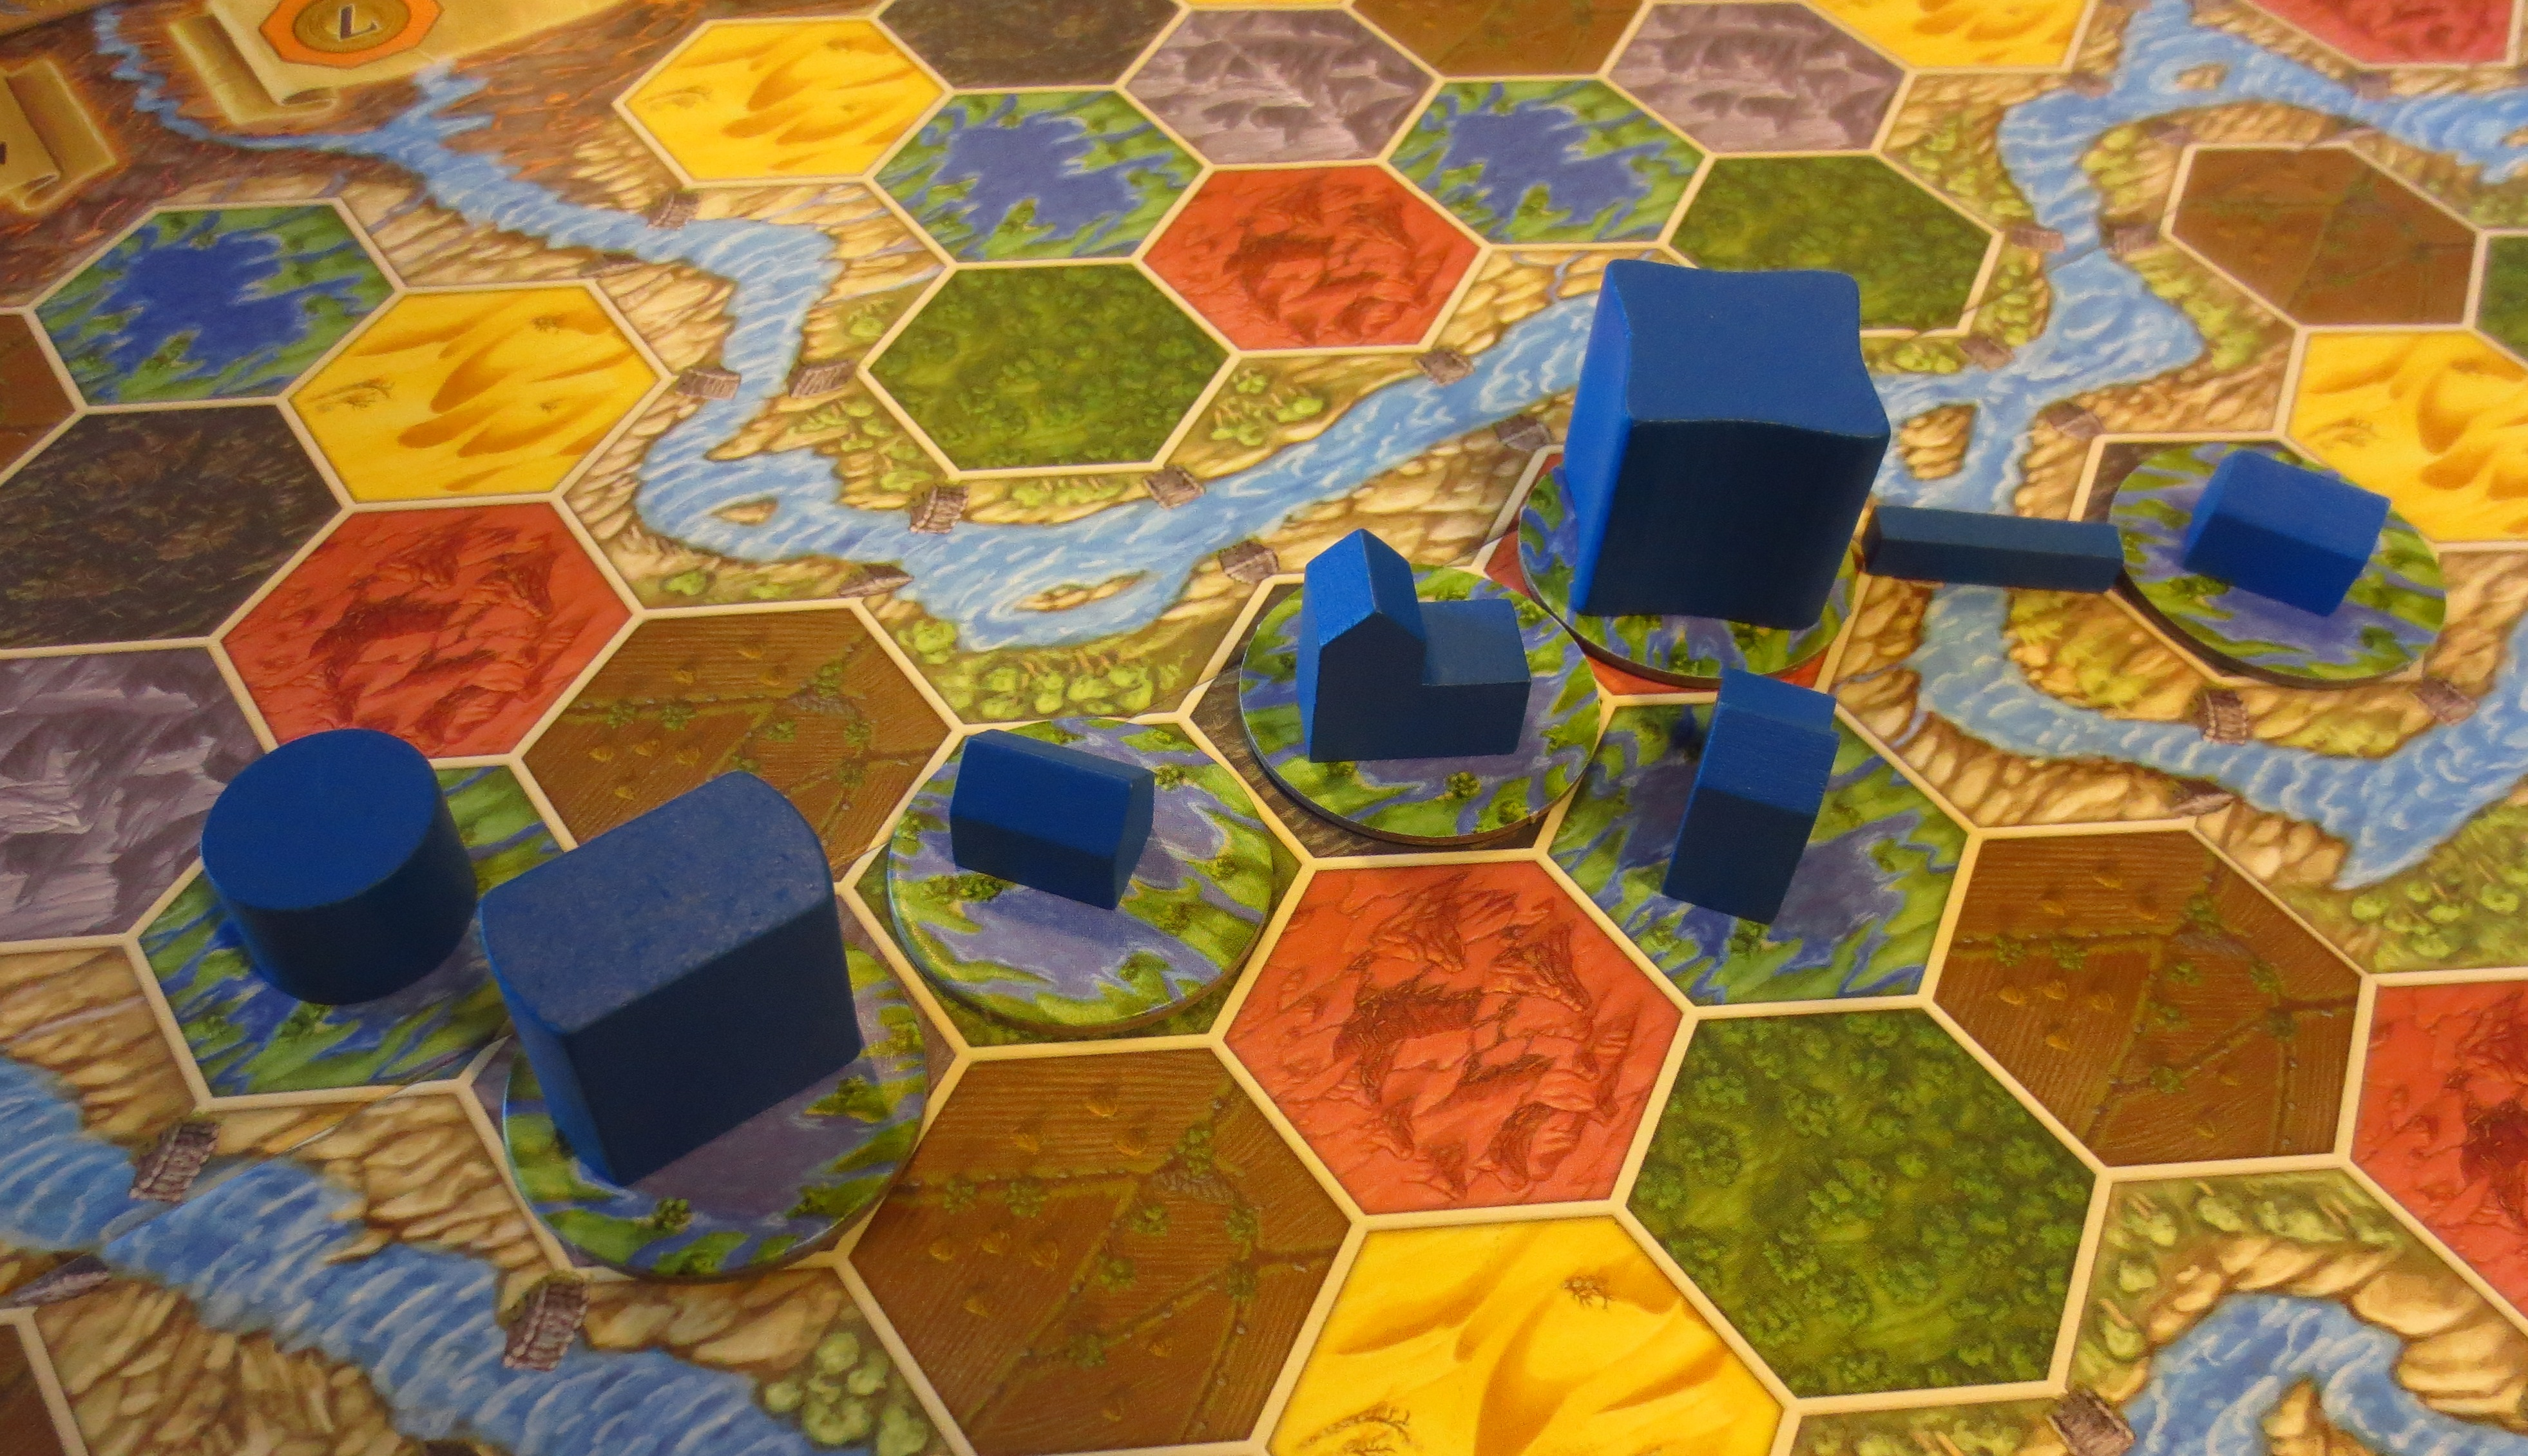
\includegraphics[width=0.5\textwidth]{Buildings}
\caption{Different shapes of buildings in Terra Mystica \label{Fig:Buildings}}
\end{figure}

When a player places a building on a tile adjacent to one already occupied by another player, the person placing the new building has to offer the other player a currency called power. The amount of power offered is based on the type of building adjacent to the new building. Furthermore, the player receiving power has to give up victory points corresponding to the amount of power received minus one. This mechanic is often forgotten in the game. With an augmentation, it would be possible for the game to remind the players involved to offer power, as well as how much power should be offered, and how many victory points are to be given up in exchange.
\begin{figure}[h!]
\centering \includegraphics[width=0.4\textwidth]{CultTracker2}
\caption{The cult tracker \label{Fig:CultTracker}}
\end{figure}

Terra Mystica has a cult track, which is a separate board which represents the players' influences with four different cults. As the game progresses, players may gain cult points, which grant them power. Furthermore, in the end of the game, players are awarded victory points based on their position on the cult track. Through an augmentation of the game, it would be possible to keep track of the cult track digitally.

The game is structured around the concept of rounds and turns. A round consists of multiple turns, taken by players in order. In one turn, the current player can take one action. Afterwards, their turn ends, and the next player takes their turn. When the last player in the turn order takes their turn, the turn then goes to the first person in the turn order. When it is a player's turn, they can choose to pass, which means they drop out of the current turn order. Then, they are not getting any more turns until the next round starts. When every player has passed in the current round, the next round starts. A full game of Terra Mystica takes six rounds to play.